\documentclass[9pt,a4paper]{extarticle}
\usepackage[utf8]{inputenc}
\usepackage[spanish]{babel}
\usepackage[top=0.25in, bottom=0.25in, left=0.4in, right=0.2in]{geometry}
\usepackage{amsmath, amssymb, amsfonts}
\usepackage{graphicx}

%letra en arial
%\usepackage{helvet}
%\renewcommand{\familydefault}{\sfdefault}

\usepackage{enumerate}% http://ctan.org/pkg/enumerate

\begin{document}
\pagenumbering{gobble}
\hrule
\center{Final de Geomtría II}
\center {Agosto de 2014}
\begin{enumerate}
    \item Dada la ecuación $\dfrac{x^2}{a^2} + \dfrac{y^2}{b^2}=2z $ se pide:
    \begin{enumerate}
        \item ¿Qué cuádrica es?
        \item Analizar las intersecciones con los ejes, los planos coordenados y los planos paralelos a los planos coordenados.
        \item Representar aproximadamente.
    \end{enumerate}
    
    \item Dados $a =-4$, $b=6$, $c=1$, hallar analítica y gráficamente el punto $d / abcd$ formen un grupo armónico.

\item Establecer y justificar la relación entre el grupo métrico y el grupo proyectivo.

\item Desarrollar brevemente cuales son las características principales de un fractal. Explicar el triángulo de Sierpinski.

\item Analizar la siguiente propiedad con elementos propios e impropios:

“Si tres o más (R) son incidentes de a dos y no están todas en un mismo (pl) pasan todas por un mismo (p)”.

\end{enumerate}
\hrule

\center{Final de Geomtría II}
\center {05/12/17}

\begin{enumerate}

\item Definir polaridad. En el gráfico dado indicar las polares con los polos respectivos.

\begin{center}
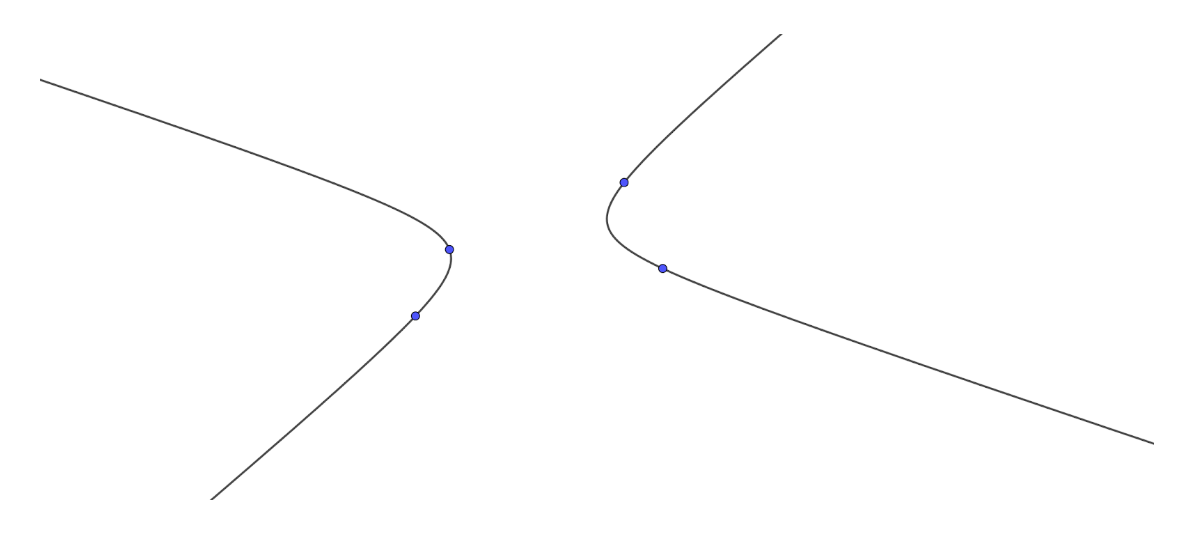
\includegraphics[scale=0.6]{51217punto1}
\end{center}


\item Indicar la ecuación de un hiperboloide de dos hojas  de eje $y$. Analizar las intersecciones      del mismo con los ejes y planos coordenados, y con  planos paralelos a los planos coordenados. Realizar un gráfico  aproximado.


\item Desarrollar brevemente cuales son las características principales  de un fractal. Explicar triángulo de Sierpinsky 


\item Demostrar  el teorema de Desargues y ejemplificarlo para el caso en que un trivértice tenga un vértice impropio y el otro tenga dos vértices impropios.

\end{enumerate}
\hrule

\center{Final de Geomtría II}
\center{5/12/16}

\begin{enumerate}
\item
    \begin{enumerate}
        \item Demostrar  el teorema de Pascal.
        \item Verificarlo en el caso de un hexágono regular inscripto en una circunferencia.
    \end{enumerate}

\item Analizar en forma completa (intersecciones con los ejes, con los planos coordenados y con planos paralelos a los planos coordenados. Gráfica)
la ecuación  $\dfrac{x^2}{a^2} + \dfrac{y^2}{b^2} + \dfrac{z^2}{c^2} = 1$

\item Definir polaridad. Hallar gráficamente  la polar de un punto en los casos que sea exterior e interior a una cónica.


\item Desarrollar brevemente cuales son las características principales  de un fractal. Explicar el copo de nieve. 

 \item Analizar con elementos propios e impropios la siguiente propiedad:

"Si un (p)  pertenece a una  (R) existe un (pl) que pasa por un (p)  y no incluye a la  (R)".

\end{enumerate}
\hrule

\newpage
\hrule
\center{Final de Geomtría II}
\center{17/7/14}

\begin{enumerate}
Escrito:


\item Hallar la ecuación general de un hiperboloide con la intersección con los planos coordenados y paralelos. Graficar aproximadamente.


\item Cónica por invariantes.


\item Hallar $k$ para una razón simple en los casos donde $a$ y $b$ son puntos fijos, y $c$ variable.


\item Dado un (p) que pertenece a una (R), existe un (pl) que pasa por (p) y que no incluye a la (R). Hallar todas las posibilidades


\item Demostrar Teorema de Desargues y verificarlo para un trivértice con dos puntos impropios y el otro con uno.

Oral:

¿Qué es un cuadrivértice constructor?

¿Cómo encontrar el cuarto armónico de manera gráfica?, etc.

\end{enumerate}
\hrule

\center{Final de Geomtría II}
\begin{enumerate}
    \item Describir las características generales de los fractales o de programa de Erlanger
\item	Alguna demostración: Desargues, Pascal o la relación entre la métrica y la proyectiva (colineación y simetría axial)
\item	Ejercicio de cuádricas: escribir una ecuación en forma general y analizarlos gráficamente (con las intersecciones con los ejes, los planos coordenados y con planos paralelos a los planos coordenados).
\item	Polar: cómo traspasar de coordenadas polares a cartesianas
\item	Ejercicio de invariantes
\item	Proyectiva: toma alguna propiedad como tomo en el parcial considerando los elementos (p), (R) y (pl) (hay que saberse los 8 axiomas).
\end{enumerate}
\hrule

\center{Final de Geomtría II}
\center{14/12/15}
\begin{enumerate}
\item Explicar el programa de Erlanger 
\item Analizar con elementos propios e impropios 
Si un (p) pertenece a una (R) existe un (pl) que pasa por un (p) y no incluye a la (R)
\item Explicar la relación entre coordenadas polares y coordenadas cartesianas
   
\begin{center}
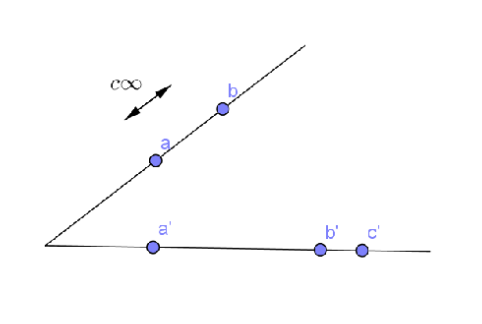
\includegraphics[scale=0.75]{141215final.png}    
\end{center}
\item Definir cónica según geometría proyectiva, ¿Cuándo es elipse, hiperbola, parabola?
\item Establecer proyectividad entre las puntuales
 \end{enumerate}
 \hrule
 \newpage
 
\hrule
\center{Final de Geomtría II}
\center{16/12/09}
\begin{enumerate}

\item Desarrollar el problema de los puentes de Konisberg

\item Analizar de forma completa 

\item Definir polaridad. Hallar gráficamente la polar de un punto en los casos que sea exterior e interior de una cónica.

\item Establecer la proyectividad entre dos puntuales

\item Establecer y demostrar la relación entre la geometría proyectiva y la métrica. 

\end{enumerate}
\hrule

\center{Final de Geomtría II}
\center{Febrero 2010}
\begin{enumerate}

\item Dada la ecuación $\dfrac{x^2}{9} + \dfrac{y^2}{25}=\dfrac{z^2}{16}+1 $ se pide:  
\begin{enumerate}
    \item ¿Qué cuádrica es?
\item Hallar las intersecciones con los ejes y planos coordenados
\item Hallar las intersecciones con $y=6$  y  $z= \pm 4$ 
\item Representar aproximadamente. 
\end{enumerate}


2) Dados $a=-4$, $b=6$ y $c=1$  y  hallar analítica y gráficamente el punto $d / abcd$ formen un grupo armónico.

3) Establecer y justificar la relación entre el grupo métrico y el grupo proyectivo.

4) Desarrollar brevemente cuales son las características principales de un fractal. Explicar el copo de nieve.

5) Enunciar el teorema de Desargues y verificarlo en un gráfico.

\end{enumerate}
\hrule

\center{Final de Geomtría II}
\center{09/12/2009}
\begin{enumerate}

\item Enunciar y demostrar el teorema de Desargues.

\item Indicar que transformaciones caracterizan a las distintas geometrías (métrica, afín, proyectiva y topológica) y explicar las relaciones entre los distintos grupos.

\item Dados $a=-5$, $b=2$ y $c=-1$ hallar gráfica y analíticamente el punto $d / abcd$ es un grupo armónico.

\item Explicar cuál es el procedimiento para desarrollar el triangulo de Sierpinski y sus características 

\item Ejemplificar en todos los casos el siguiente axioma: 

Si una (R) esta incluida en un (pl) existe algún (p) que pertenece a (pl) tal que no pertenece a (R)

\end{enumerate}
\hrule

\center{Final de Geomtría II}
\center{2006}
\begin{enumerate}

\item Establecer la proyectividad entre dos puntuales.

\item Desarrollar brevemente cuáles son las características principales del fractal de Koch.

\item
\begin{enumerate}
    \item Enunciar y demostrar el teorema de Pascal. 
    \item Verificarlo en el caso de un hexágono regular inscripto en una circunferencia.
\end{enumerate}

\item Demostrar que la suma de dos razones dobles que difieren por la permutación de los elementos medios es uno.

\item Definir cónica punto.

\end{enumerate}
\hrule
\newpage
\hrule
\center{Final de Geomtría II}
\center{17/12/18}
\begin{enumerate}

\item Indicar la ecuación de un hiperboloide de dos hojas y analizar las intersecciones del mismo con los ejes y planos coordenados, y con planos paralelos a los planos coordenados. Realizar un gráfico aproximado.

\item Enunciar y demostrar el teorema de Desargues.

\item Analizar por invariantes $2x^2 + 4xy - 6y^2-3x+7y-2=0$

\item Realizar una comparación entre geometrías euclideanas y no euclideanas.

\item Definir polaridad. Indicar gráficamente, en el siguiente gráfico, las polares y sus respectivos polos.
\begin{center}
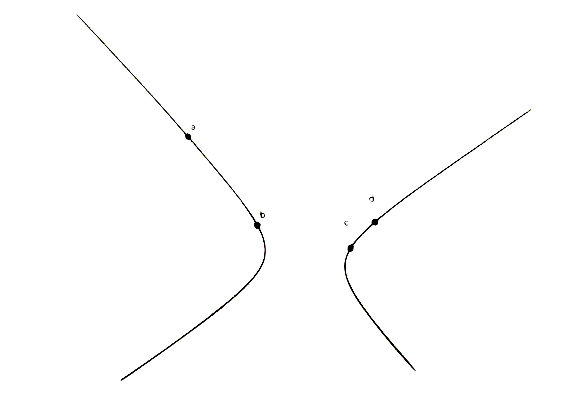
\includegraphics[scale=0.6]{graffinal18.png}
\end{center}

\end{enumerate}
\hrule
\end{document}